\chapter{Project: Soap Bubble Shader}
\label{cha:proj-udvid-af}


\section{Introduction}
\label{sec:proj-intro}

Development steps of soap bubble shader and visualisations of the results are presented in this report. Decision, design, implementation phases of the project are described. \\

For this project Andrew Glassner's Notebook \cite{Glassner:1999:AGN:318952} is the most dominant source of influence. 



\section{Motivation \& Process}
\label{sec:proj-motiv}
Among the exercises, exercise 10 was the one that makes me entertained, encouraged and inspired. I decided to extend the exercise by implementing a new, unusual shader and a chromatic glass shader as I was instructed. After I completed the chromatic glass shader, I made a research on internet to figure out which shader I should do. I came up with idea of introducing a bubble shader after a while.\\
I tried to understand the nature of a soap bubble, the physics behind it and I analyzed the implementation ideas, previous work that was done by others. Once I felt I gathered the background information needed for the project, I moved on implementation phase of bubble shader.


\section{The Basis for Application Program}
\label{sec:proj-basis}
I copied entire project of exercise 10 and removed the shaders and the functionalities which is not needed for this task except one: glass shader.\\
Bubble is a just a surface, very thin surface in the shape of sphere, encapsulating some air. Since the width of this shell is not more than few micrometers, the refraction of a soap bubble is zero. Therefore a soap bubble can be considered as a glass globe made by a special type of glass refraction index of which is equal to the one of air. I have chosen glass shader as a basis for my project.\\


\section{The Bubble Shader}
\label{sec:proj-shad}

As stated in Section \ref{sec:proj-basis}, there is no refraction in bubble. So I skip refraction lookup procedure. Instead, I simply assign incident vector to resulting refraction vector. The resulting scene can be seen in Figure \ref{fig:report-1}.

\begin{figure}[hp]
\centering
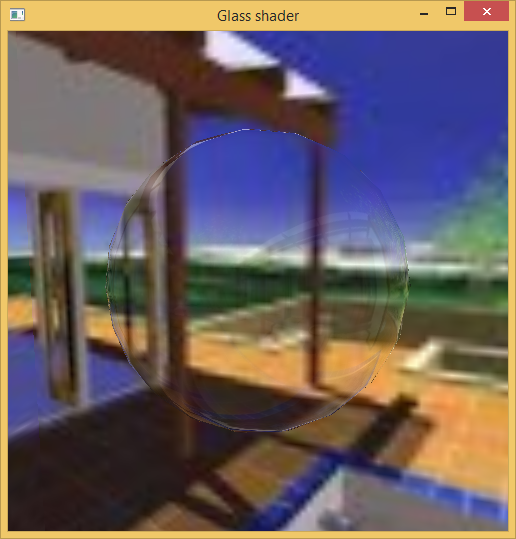
\includegraphics[width=8cm]{../Screenshots/report/1.png}
\caption{Transparent sphere without refraction phenomena}
\label{fig:report-1}
\end{figure}


The name of phenomena that gives a colorful appearance to bubble is called \emph{iridescence}. Since a bubble is actually a thin film of soap-water mixture, the rays coming to the bubble reflect two times. The light rays reflects once from outer surface of the film and inner surface of the film. The width of the bubble shell is so small that these two reflections of photons interferes with each other, resulting \emph{iridescence}.\\
Simulation of this natural phenomena in computer is possible by using the formula of reflection in bubble surface \cite[p.~107]{Glassner:1999:AGN:318952}:

\begin{equation}
I_{r} = 4I_{i}R_{f} \sin^2(\frac{2\pi}{\lambda}w\eta\cos{\theta_{t}})
\end{equation}

where \emph{$I_{r}$} is the intensity of reflecting light, \emph{$R_{f}$} is fresnel term that we are familiar with in glass shader,  \emph{$I_{i}$} is the intensity of incoming light, \emph{$\lambda$} is wavelength of incoming light ray in nanometers, \emph{w} is width of soap bubble in nanometers, \emph{$\eta$} is ratio between refraction index of air and that of bubble shell (refraction index of bubble shell is assumed 1.33, the same with that of water), \emph{$\theta_{t}$} is the angle of transmission in bubble shell. \\

I use Schlick's Approximation method \cite{Schlick94aninexpensive} to calculate fresnel term.

After some experiments in application to determine ideal bubble width, I notice that a bubble with 2400 nm width appears realistic to human. Reader should consider that previous comments are quite subjective.\\


I make calculation of \emph{$I_{r}$} for three main color; red, green and blue. I fuse single calculations for these three colors which resulted in the final term for iridescent reflection.\\

The resulting screenshot of scene can be seen in Figure \ref{fig:report-2}.

\begin{figure}[hp]
\centering
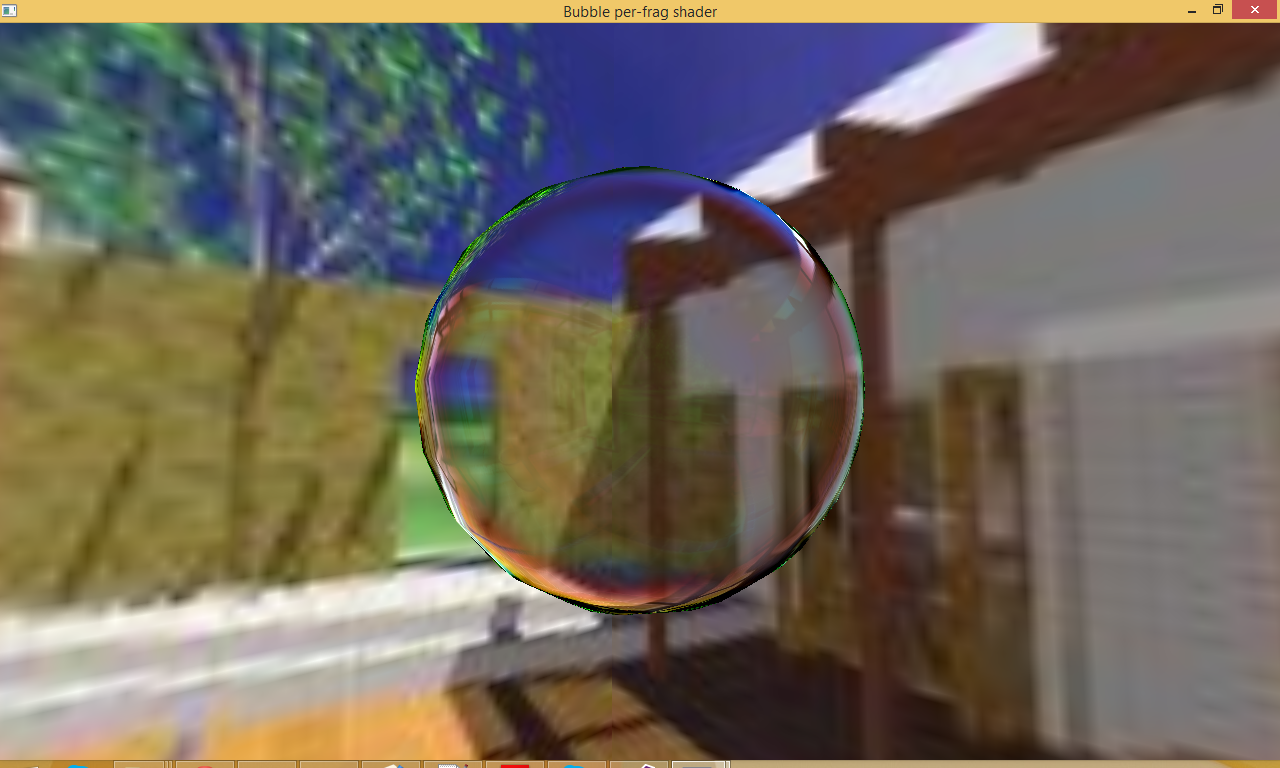
\includegraphics[width=8cm]{../Screenshots/report/2.png}
\caption{Bubble shader. Per-fragment shading.}
\label{fig:report-2}
\end{figure}

As a functionality, I add per-vertex and per-fragment bubble shader to the project. You can toggle between shaders by pressing \emph{s} key. Per-vertex bubble shader can be seen in Figure \ref{fig:report-3}. The difference between two shading strategies are noticeable. \\


\begin{figure}[hp]
\centering
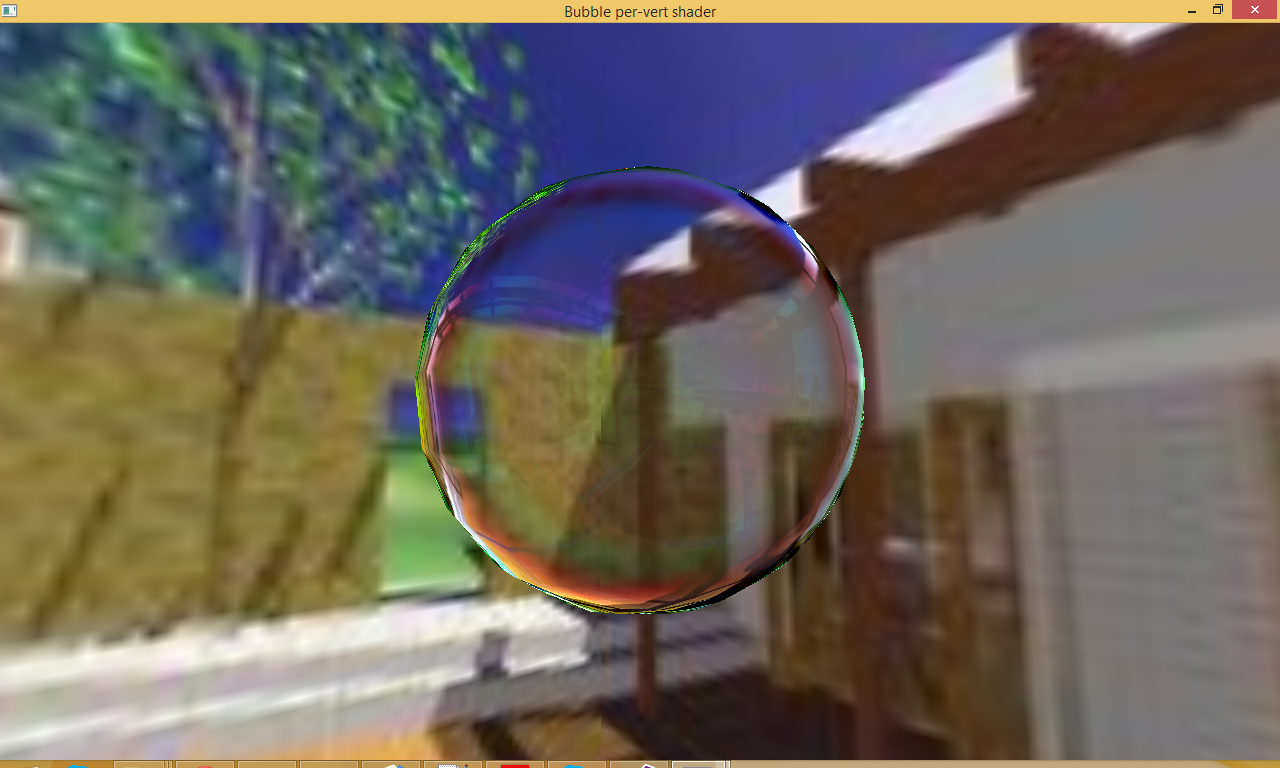
\includegraphics[width=8cm]{../Screenshots/report/3.png}
\caption{Bubble shader. Per-vertex shading.}
\label{fig:report-3}
\end{figure}


%%% Local Variables:
%%% mode: latex
%%% TeX-master: "report_main"
%%% End: 